\chapter[~]{Вивчення додаткових можливостей програми для розробки креслень sPlan}

\textbf{Мета роботи} --- ознайомитись з додатковими можливостями програми для розробки креслень схем
sPlan, навчитись працювати з формами документів, створювати власні елементи та бібліотеки
компонентів.

\section{Виконання креслення основного напису для креслення}

\begin{enumerate}[leftmargin=*]
\item Для початку роботи потрібно встановити книжну орієнтацію аркуша, та переконатись що задані
  параметри аркуша відповідають поставленому завданню. Для цього переходимо в меню ``Лист'' >
  ``Свойства листа'' (\ref{fig:document_settigns}). 

\begin{figure}[!ht]
  \centering
  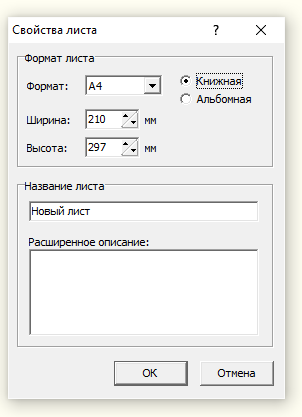
\includegraphics[]{./images/lab2/document_settings.png}
  \caption{Вікно налаштувань аркуша}
  \label{fig:document_settigns} 
\end{figure}

\newpage

\item Задаємо початкові розміри аркуша використовуючи інструмент ``Розміри''. (\ref{fig:dimentions})
  
\begin{figure}[!ht]
  \centering
  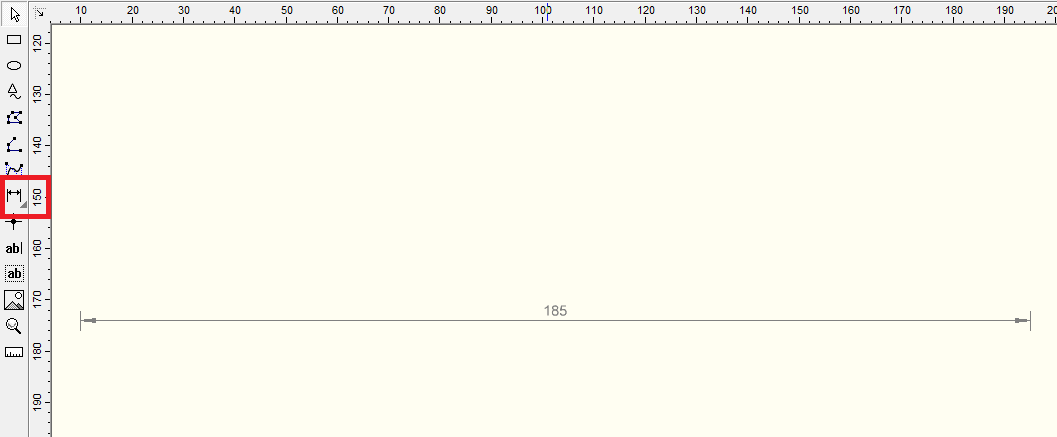
\includegraphics[width=0.9\linewidth]{./images/lab2/dimentions.png}
  \caption{Інструмент ``Розміри''}
  \label{fig:dimentions} 
\end{figure}

\item Використовуючи інструмент ``Прямокутник'' будуємо зовнішню рамку. (\ref{fig:rectangle})
  
\begin{figure}[!ht]
  \centering
  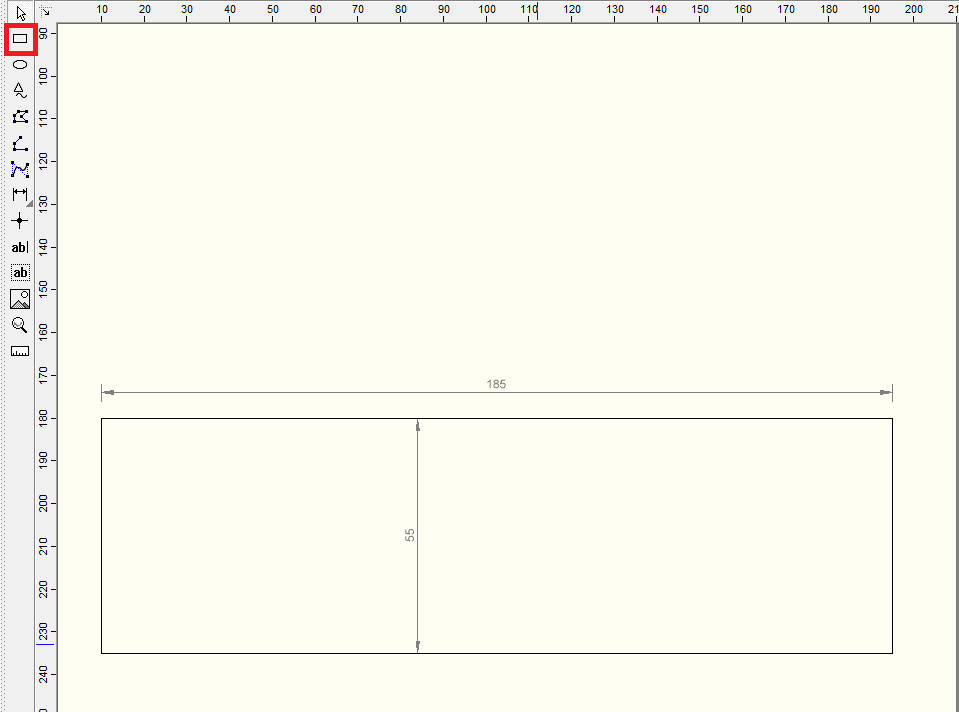
\includegraphics[width=0.9\linewidth]{./images/lab2/first_step.png}
  \caption{Інструмент ``Прямокутник''}
  \label{fig:rectangle} 
\end{figure}

\item Використовуючи вище наведені інструменти задаємо розміри та будуємо праву частину основного
  напису. (\ref{fig:rectangle})
  
\begin{figure}[!ht]
  \centering
  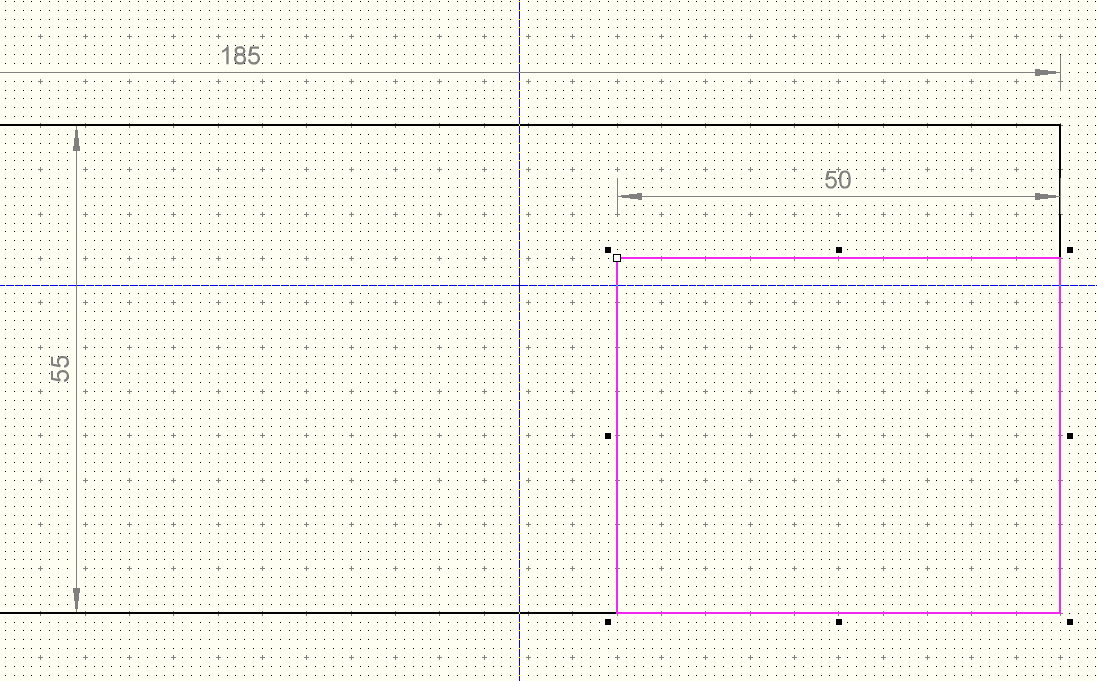
\includegraphics[width=0.9\linewidth]{./images/lab2/second_step.png}
  \caption{\label{fig:second_step}}
\end{figure}
\begin{figure}[!ht]
  \centering
  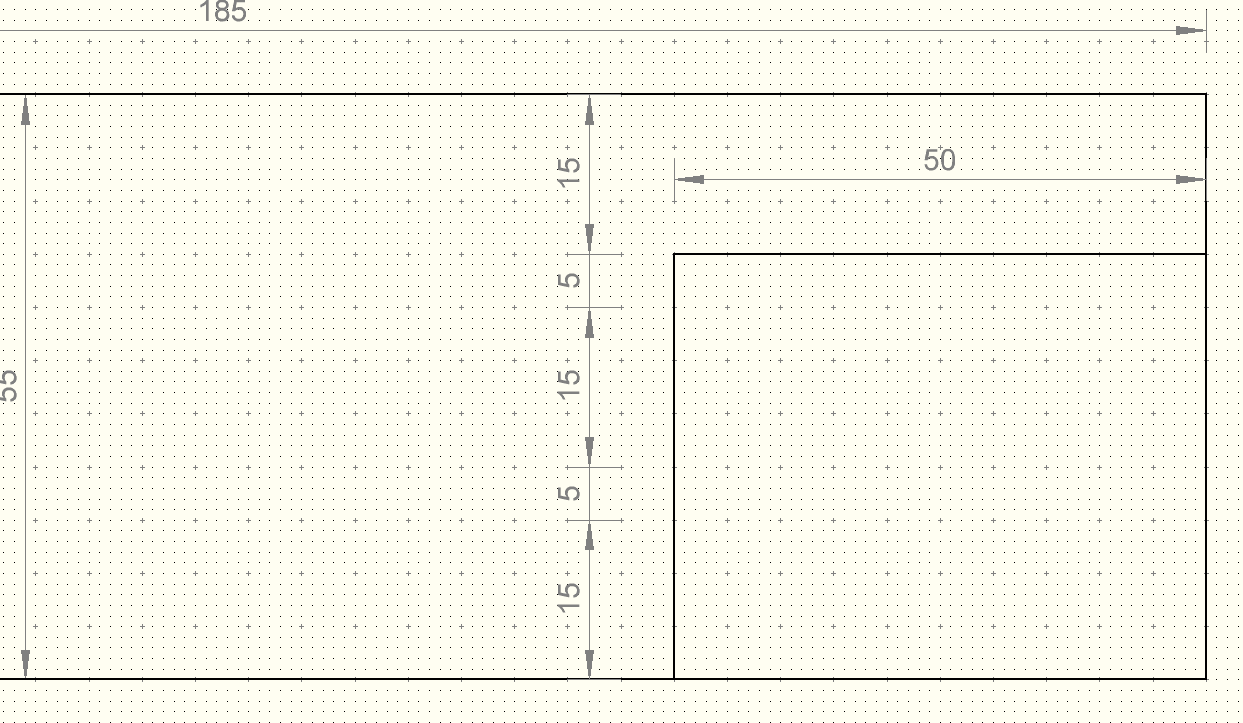
\includegraphics[width=0.9\linewidth]{./images/lab2/third_step.png}
  \caption{\label{fig:third_step}}
\end{figure}

\FloatBarrier

\item Застосуємо інструмент лінія, для побудови відповідних горизонтальних та вертикальних ліній. (\ref{fig:line})
  \begin{figure}[!htb]
  \centering
  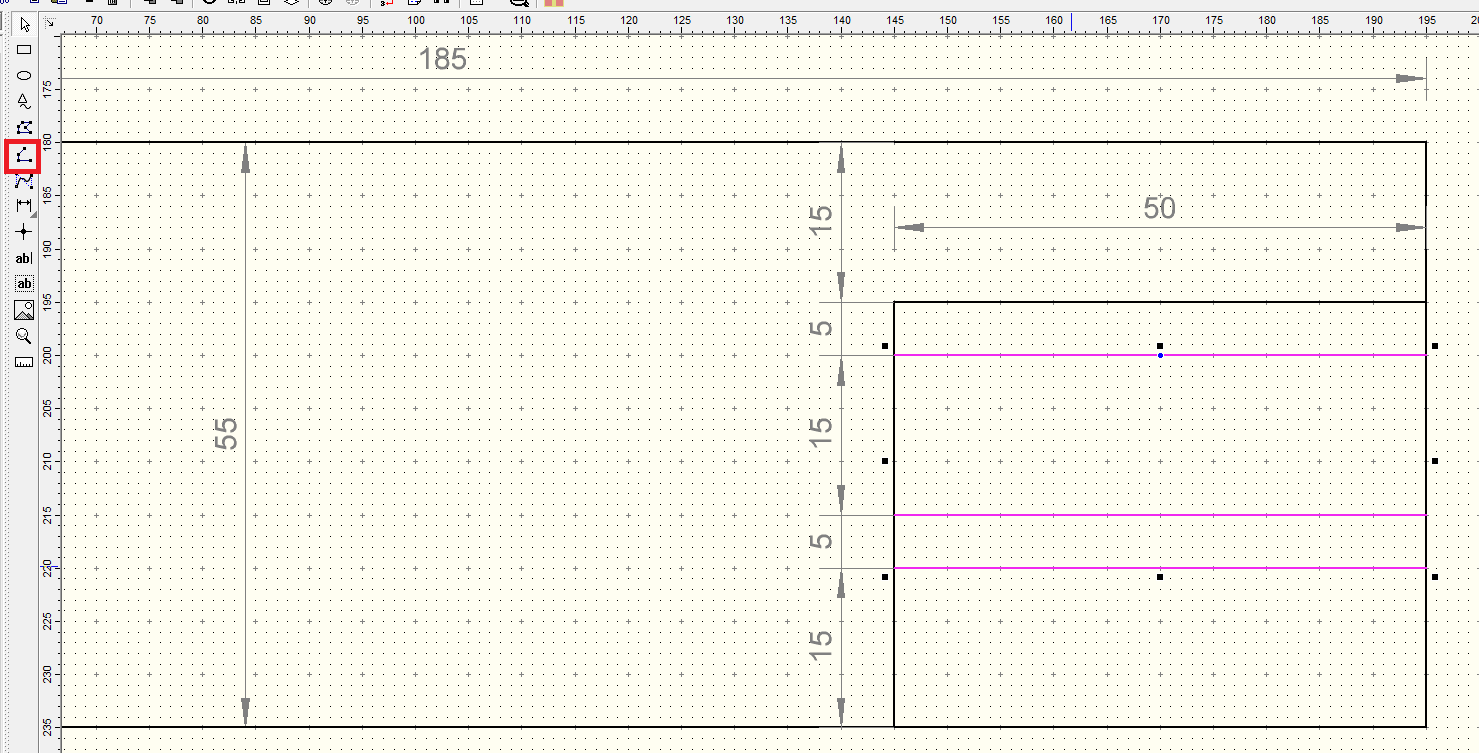
\includegraphics[width=0.9\linewidth]{./images/lab2/fourth_step.png}
  \caption{Інструмент ``Лінія''}
  \label{fig:line}
\end{figure}
\FloatBarrier

\item Добудовуємо залишок основного напису використовуючи вказані інструменти
  \begin{figure}[!htb]
  \centering
  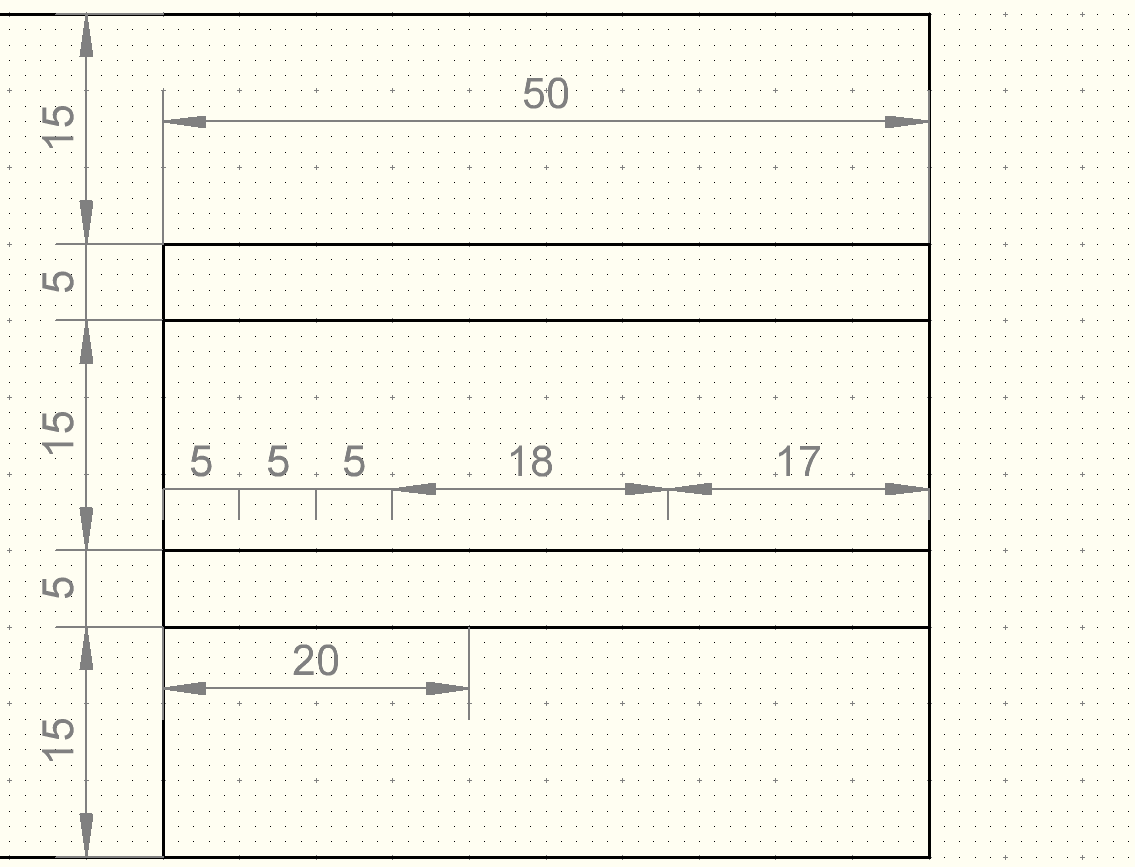
\includegraphics[width=0.9\linewidth]{./images/lab2/fifth_step.png}
  \caption{ \label{fig:fifth_step}}
\end{figure}
\begin{figure}[!htb]
  \centering
  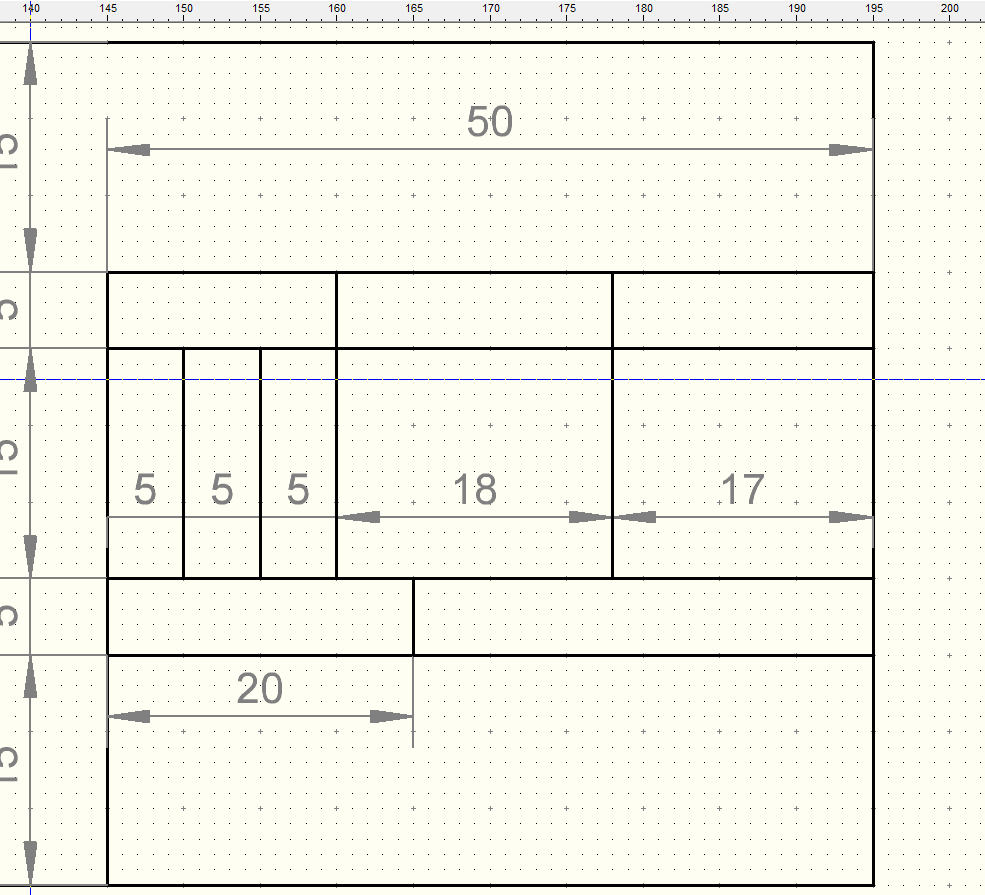
\includegraphics[width=0.9\linewidth]{./images/lab2/sixth_step.png}
  \caption{}
  \label{fig:sixth_step} 
\end{figure}
\begin{figure}[!htb]
  \centering
  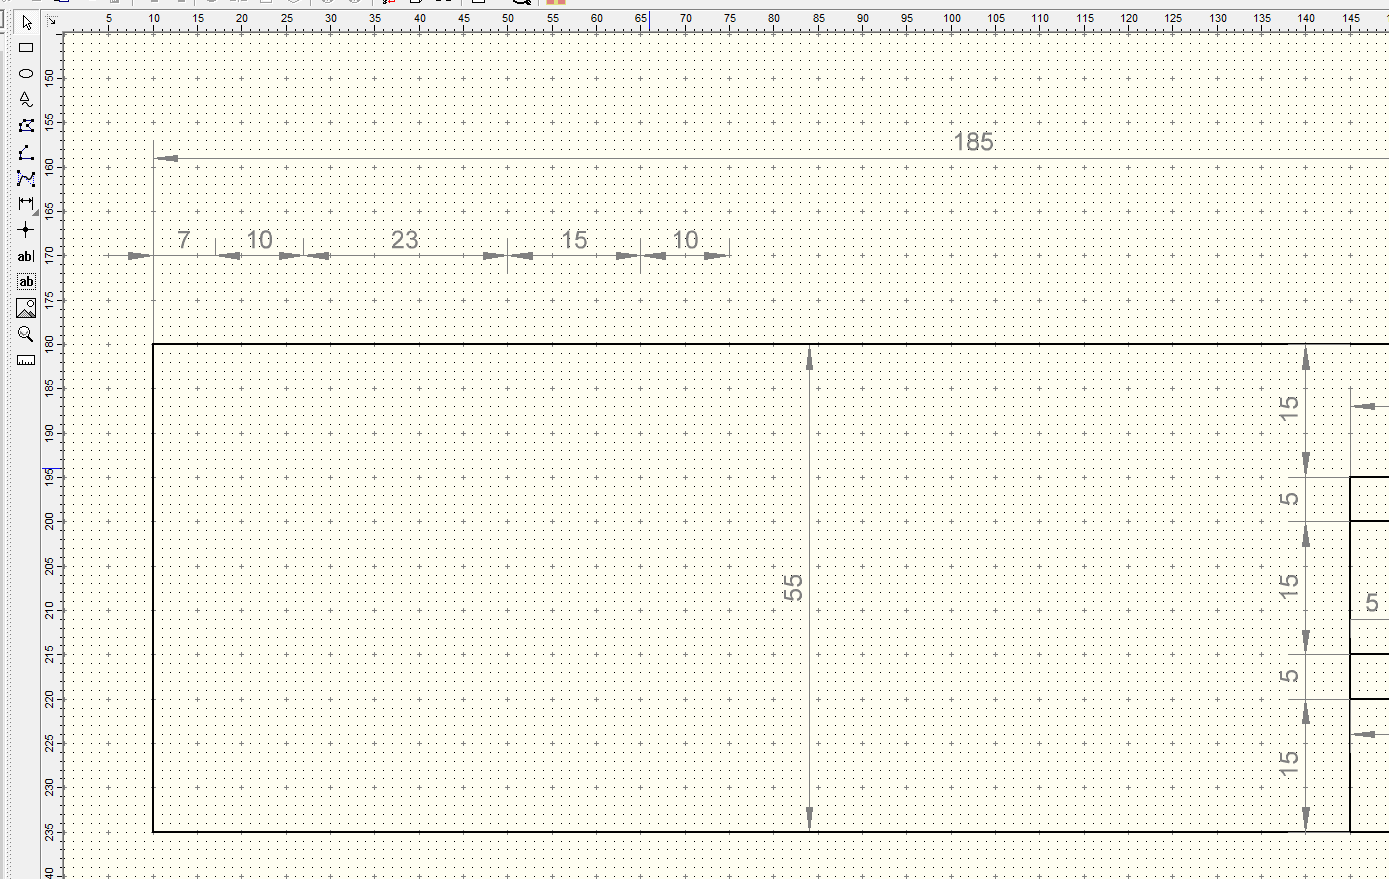
\includegraphics[width=0.9\linewidth]{./images/lab2/seventh_step.png}
  \caption{}
  \label{fig:seventh_step} 
\end{figure}
\begin{figure}[!htb]
  \centering
  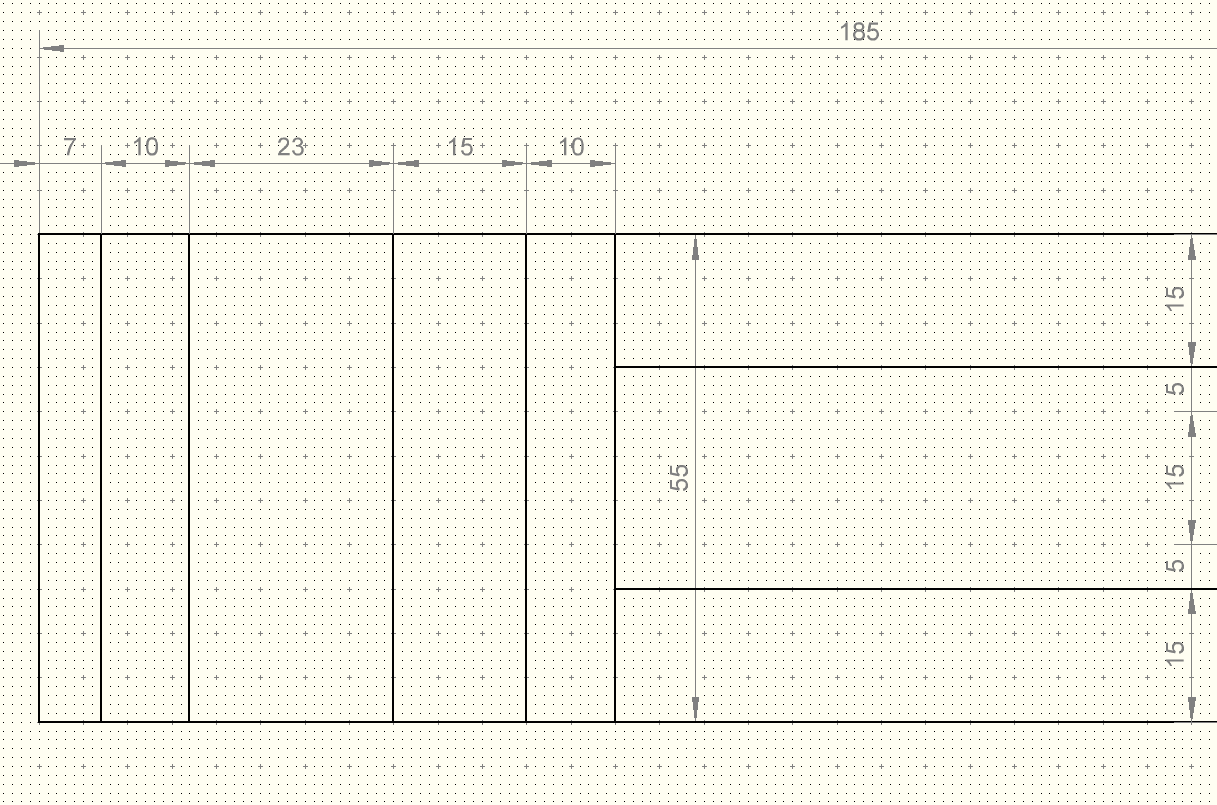
\includegraphics[width=0.9\linewidth]{./images/lab2/eighth_step.png}
  \caption{}
  \label{fig:eigth_step} 
\end{figure}
\begin{figure}[!htb]
  \centering
  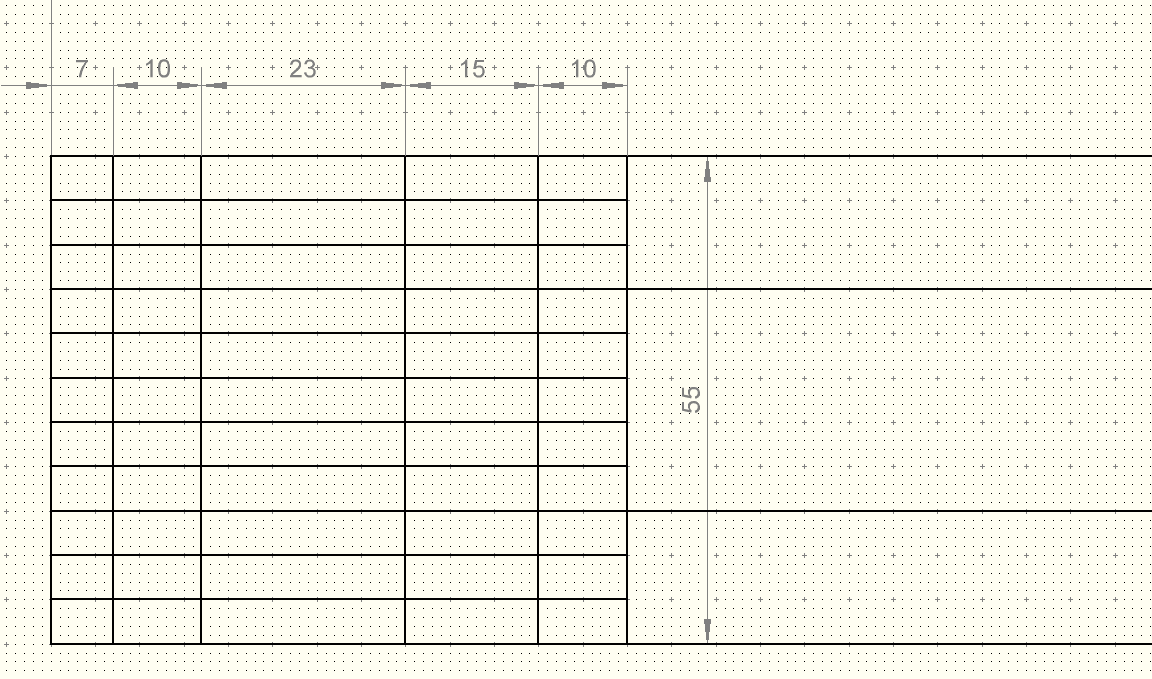
\includegraphics[width=0.9\linewidth]{./images/lab2/nineth_step.png}
  \caption{}
  \label{fig:nineth_step} 
\end{figure}

\FloatBarrier
\item Виділивши необхідні лінії натискаємо праву клавішу мишки та обираємо пункт ``Свойства'' в
  якому задаємо необхідну товщину лінії.
  \begin{figure}[!htb]
  \centering
  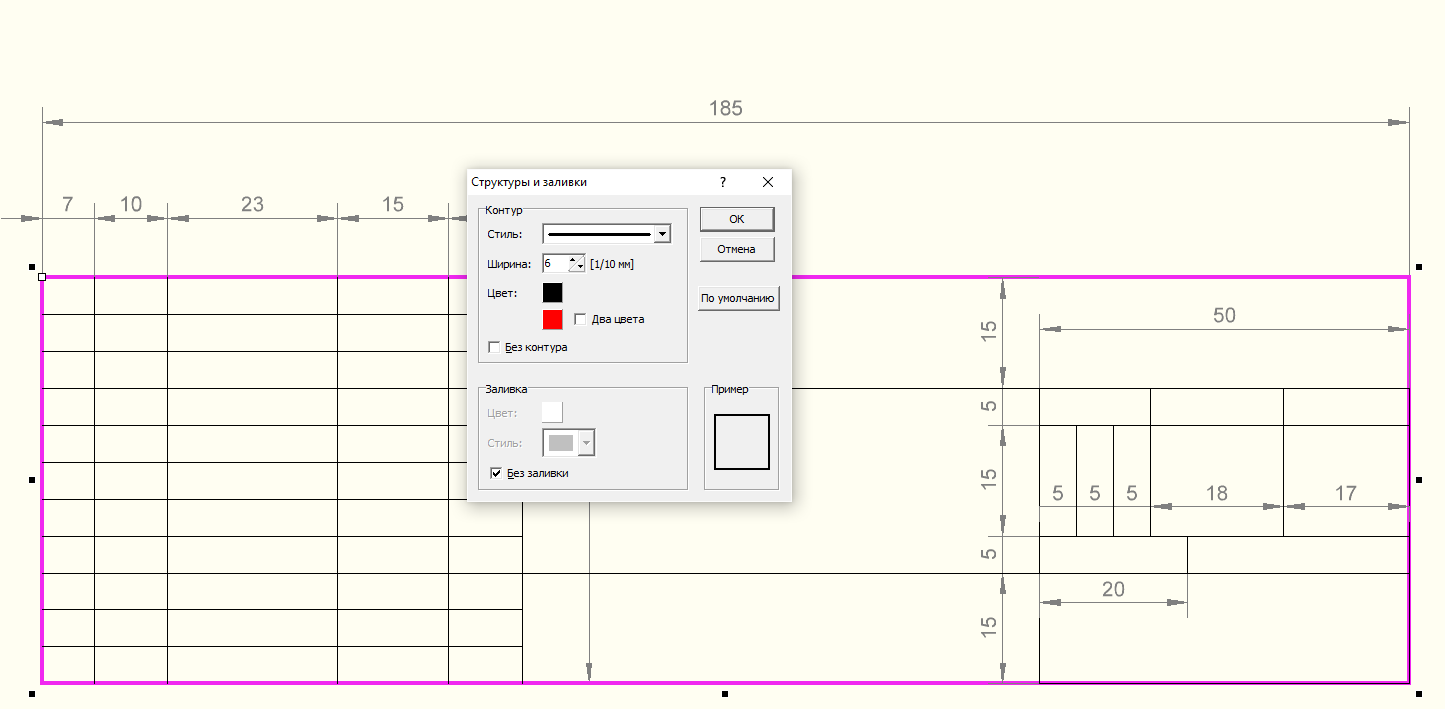
\includegraphics[width=0.9\linewidth]{./images/lab2/bold_line.png}
  \caption{}
  \label{fig:nineth_step}
\end{figure}
\FloatBarrier
  
\end{enumerate}

\FloatBarrier
\section{Створення користувацьої бібліотеки елементів}

\section{Виконання крелсення елементів електронної схеми за варіантом}

\section{Виконання креслення електронної принципової схеми з використанням створених елементів}

\section{Створення переліку  елементів схеми}

